%%%%%%%%%%%%%%%%%%%%%%%%%%%%%%%%%%%%%%%%%%%%%%%%%%%%%%%%%%%%%%%%%%% 
%                                                                 %
%                            CHAPTER                              %
%                                                                 %
%%%%%%%%%%%%%%%%%%%%%%%%%%%%%%%%%%%%%%%%%%%%%%%%%%%%%%%%%%%%%%%%%%% 
\chapter{Planning}
\section{Herwerkte planning \ref{fig:plan}}
\begin{figure}[!ht]
	\centering
	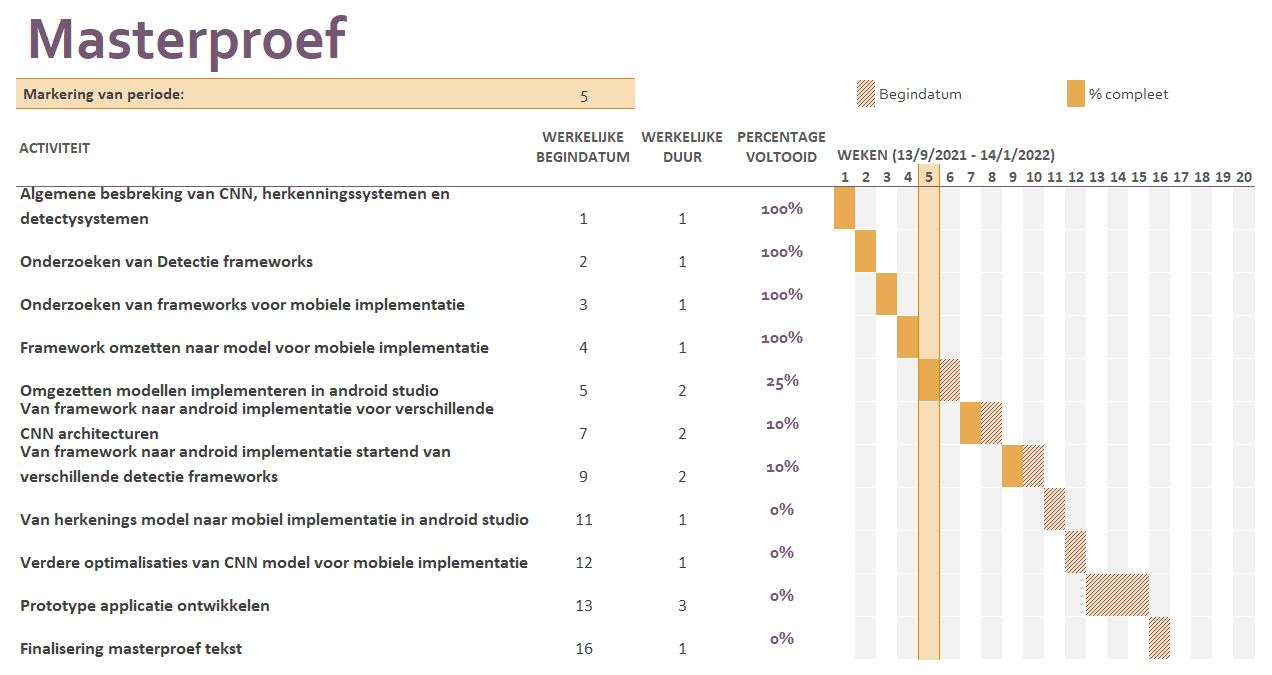
\includegraphics[width=1.0\linewidth]{fig/planning.jpg}
	\caption{herwerkte planning.}
	\label{fig:plan}
\end{figure}
\section{ResNet50 resultaten}
Het ResNet50 model van TensorFlow kan eenvoudig geconverteerd worden naar ONNX en TFlite.
De TFLite implementatie in Android studio is bijzonder gemakkelijk door het toevoegen van Metadata waardoor de code voor de Android studio implementatie voor ons wordt gegenereerd.
Het ResNet50 model van PyTorch kan ook eenvoudig geconverteerd worden naar ONNX en PyTorch Mobile.
De Android studio implementatie is ook eenvoudig uit te voeren door de PyTorch Mobile documentatie te volgen.
%De ONNX implementatie in Android studio was ook stap voor stap de ONNX documentatie volgen.
Wel moet er voor ONNX opgelet worden dat de input correct wordt genormaliseerd en dat de input het juiste formaat heeft (NCWH of NWHC) afhankelijk van het originele framework.
Voor het uitvoeren van de modellen gebruiken we Google Colaberate met een CPU runtime en het mobiel toestel Xiaomi T9.


In tabel \ref{tab:class_size} kunnen we de bestandsgrootte zien van elk model.
Hierbij kunnen we geen duidelijk onderscheid maken tussen TensorFlow en PyTorch.
Wel kunnen we zien dat na het converteren naar ONNX of een mobiel model de bestandsgrootte met enkel KB verkleint.
\begin{table}[!ht]
    \caption{Binaire grootte van al de ResNet50 modellen}
\begin{tabular}{cccc}
    \hline
    Framework & Standaard model & Mobiel model & ONNX model \\
    \hline
    TensorFlow & 98.3MB & 97.45MB & 97.44MB \\
    PyTorch & 97.81MB & 97.44MB & 97.4MB \\
    \hline
\end{tabular}
\label{tab:class_size}
\end{table}

Voor de latency zien we dat bij de uitvoering op het mobiele toestel, het PyTorch model de snelste uitvoering heeft.
Over het algemeen is het PyTorch model sneller enkel bij de uitvoering van ONNX model.
Ondanks dat het ONNX model voor zowel PyTorch als TensorFlow de snelste uitvoering heeft in Google Colaberate zien we dat dit niet het geval is bij de uitvoering op het mobiele toestel.

\begin{table}[!ht]
    \caption{Uitvoersnelheid van de ResNet50 modellen in Google Colab en in de mobiele omgeving. Als mobiele omgeving gebruiken we de Xiaomi T9.}
\begin{tabular}{cccccc}
    \hline
    Framework & Standaard model & Mobiel model Colab & Mobiel model T9 & ONNX Colab & ONNX T9\\
    \hline
    TensorFlow & 0.276s & 0.405s & 0.356s & 0.106s & 0.394s \\
    PyTorch & 0.262s & 0.390s & 0.303s & 0.129s & 0.414s \\
    \hline
\end{tabular}
\label{tab:class_speed}
\end{table}

Voor de evaluatie hebben we gebruik gemaakt van de ImagenetV2-matched-frequency dataset (\cite{recht2019imagenet}).
Hierbij zien we dat enkel bij het PyTorch ONNX model de accuraatheid daalt.
In elke andere situatie blijft de accuraatheid van het model hetzelfde.

\begin{table}[!ht]
    \caption{Top 1 accuraatheid voor het standaard, mobiel en ONNX model.}
\begin{tabular}{cccc}
    \hline
    Framework & Standaard model & Mobiel model & ONNX model \\
    \hline
    TensorFlow & 37.1\% & 37.1\% & 37.1\%  \\
    PyTorch & 17\% & 17\% & 10.4\%  \\
    \hline
\end{tabular}
\label{tab:class_acc}
\end{table}

\subsection{Faster-RCNN resultaten}
Het uitvoeren van een Faster-RCNN model op een mobiel apparaat is heel wat complexer dan het ResNet50 model.
TensorFlow zit met de complexiteit dat de converter al de waarden van de verwachte outputgrootte op \'e\'en zet.
Waardoor we telkens de outputbuffers moeten defini\"eren in Android studio.
PyTorch heeft dit probleem echter niet.
Maar om het Faster-RCNN model uit te voeren in Android studio moet de Torchvision\_ops bibliotheek op een alternatieve manier ge\"importeerd worden.
Verder kan PyTorch ook niet het Faster-RCNN verder optimaliseren voor mobiel gebruik.
Aan de hand van de onderstaande resultaten zien we dat het TensorFlow Faster-RCNN model betere resultaten levert voor de uitvoersnelheid en de bestandsgrootte.

In tabel \ref{tab:rcnn_size} zien we duidelijk dat de bestandsgrootte van het PyTorch model aanzienlijk groter is dan het TensorFlow model.
Wat als gevolg heeft dat het PyTorch model te groot is om als een ONNX model uit te voeren in Android studio.
\begin{table}[!ht]
    \caption{Bestandgrootte van de verschillende Faster-RCNN modellen}
\begin{tabular}{cccc}
    \hline
    Framework & Standaard model & Mobiel model & ONNX model \\
    \hline
    TensorFlow & 115.48MB & 110.37MB & 111.88MB \\
    PyTorch & 159.8MB & 159.94MB & 159.59MB \\
    \hline
\end{tabular}
\label{tab:rcnn_size}
\end{table}

In tabel \ref{tab:rcnn_speed} zien we dat het TensorFlow model sneller wordt uitgevoerd dan het PyTorch model op het mobiel apparaat.
Ook zien we voor TensorFlow dat ONNX beter presteert dan TFLite in Google Colaborate.
Maar in de mobiele omgeving zien we dat ONNX minder snel resultaten levert dan het TFLite model.
\begin{table}[!ht]
    \caption{De uitvoer snelheid van de modellen in Google Colab en in de mobiele omgeving. Als mobiele omgeving gebruiken we de Xiaomi T9.}
\begin{tabular}{cccccc}
    \hline
    Framework & Standaard model & Mobiel model Colab & Mobiel model T9 & ONNX Colab & ONNX T9\\
    \hline
    TensorFlow & 3.617s & 5.91s & 8.33s & 4.774s & 12.388s \\
    PyTorch & 4.707s & 5.119s & 11.194s & 4.065s & / \\
    \hline
\end{tabular}
\label{tab:rcnn_speed}
\end{table}

In tabel \ref{tab:rcnn_acc} is te zien dat voor de twee frameworks de conversie geen invloed heeft op de accuraatheid.
Het standaard model, het mobiel model en het ONNX model geven hetzelfde resultaat bij zowel TensorFlow als PyTorch.
Als test data hebben we de COCO 2017 dataset genomen en de mean avarage precision bepaalt met iou \textgreater 0.5.
%% MEAN AVARAGE PRECISION
\begin{table}[!ht]
    \caption{Mean avarage precision van de modellen uitgevoerd op Google Colab en Xiaomi T9.}
\begin{tabular}{cccc}
    \hline
    Framework & mAP Standaard model & mAP Mobiel model & mAP ONNX model\\
    \hline
    TensorFlow & 0.8 & 0.8 & 0.8 \\
    PyTorch & 0.8 & 0.8 & 0.8 \\
    \hline
\end{tabular}
\label{tab:rcnn_acc}
\end{table}

\subsection{YOLO resultaten}
Zowel voor TensorFlow als PyTorch is het nodig om het YOLO model eerst te defini\"eren en vervolgens de gewichten in te laden.
Enkel het TensorFlow model kan succesvol naar een mobiel model worden geconverteerd.
Bij het TensorFlow model moet, zoals bij Faster-RCNN, de input eerst speciefiek aan het model worden toegevoegd.
In de resultaten kunnen we vaststellen dat het PyTorch model na conversie het model zeer sterk optimaliseerd.
Met een zeer negatief gevolg op de accuraatheid.

Voor de bestandsgroottes die in tabel \ref{tab:yolo_size} beschreven zijn kunnen we zien dat de standaardgrootte van het YOLO model vrij groot is.
En voor TensorFlow blijft de bestandsgrootte ongeveer hetzelfde na de conversie naar TFLite en ONNX.
Bij PyTorch zien we dat de bestandsgrootte van het model met een zeer grote factor verkleint.
De optimalisatie functie zal de meeste parameters als overbodig registreren vermits de output altijd hetzelfde is ongeacht de input.
\begin{table}[!ht]
    \caption{Binaire grootte van al de YOLO modellen}
\begin{tabular}{cccc}
    \hline
    Framework & Standaard model & Mobiel model & ONNX model \\
    \hline
    TensorFlow & 237.17MB & 236.27MB & 236.28MB \\
    PyTorch & 236.72MB & 3.55MB & 4.37MB \\
    \hline
\end{tabular}
\label{tab:yolo_size}
\end{table}

Voor de snelheid zien we in tabel \ref{tab:yolo_speed} we duidelijk een verbetering in vergelijking met het Faster-RCNN model \ref{tab:rcnn_speed}.
Door het verwijderen van al de operaties die geen invloed hebben op het resultaat zal het PyTorch model zeer snel worden uitgevoerd.
Het model zal wel altijd het zelfde resultaat voorspellen.
\begin{table}[!ht]
    \caption{De uitvoer snelheid van de modellen in Google Colab en in de mobiele omgeving. Als mobiele omgeving gebruiken we de Xiaomi T9.}
\begin{tabular}{cccccc}
    \hline
    Framework & Standaard model & Mobiel model Colab & Mobiel model T9 & ONNX Colab & ONNX T9\\
    \hline
    TensorFlow & 2.545s & 2.220s & 2.47s & 0.107s & / \\
    PyTorch & 1.441s & 0.0097s & 0.0278s & / & / \\
    \hline
\end{tabular}
\label{tab:yolo_speed}
\end{table}

In tabel \ref{tab:yolo_acc} kunnen we zien dat de conversie naar ONNX en TFLite geen invloed heeft op de accuraatheid.
Het geconverteerd PyTorch model geeft echter geen goed resultaat vermits het resultaat altijd hetzelfde is.
\begin{table}[!ht]
    \caption{Top 1 accuraatheid van de standaard en modellen voor mobiel gebruik.}
\begin{tabular}{cccc}
    \hline
    Framework & mAP Standaard model & mAP Mobiel model & mAP ONNX model \\
    \hline
    TensorFlow & 1.0 & 1.0 & 1.0 \\
    PyTorch & 0.75 & 0.0 & / \\
    \hline
\end{tabular}
\label{tab:yolo_acc}
\end{table}

De reden waarom het geconverteerd PyTorch model slechte resultaten levert is omdat de jit.trace functie een foutief resultaat levert.
Het enige wat het TorchScript model nog produceert zijn de bounding boxes van de input die we hebben meegegeven met de jit.trace functie.
Dit is vervolgens ook de reden waarom de mobiele optimalisatie van PyTorch een groot effect heeft op de bestandsgrootte.
De meeste waarden van het model worden als constant beschouwd omdat het model altijd dezelfde output levert ongeacht de input.
Dit zouden we kunnen oplossen door al de lagen apart te defini\"eren in \'e\'en methode zonder het inlezen van de configuratie file.
Vervolgens zou het mogelijk moeten zijn om dit model te converteren vermits al de gebruikte operaties een mobiel equivalent hebben.
